
% This LaTeX was auto-generated from an M-file by MATLAB.
% To make changes, update the M-file and republish this document.

\documentclass{article}
\usepackage{graphicx}
\usepackage{color}

\sloppy
\definecolor{lightgray}{gray}{0.5}
\setlength{\parindent}{0pt}

\begin{document}

    
    \begin{verbatim}
% The 2.5th and 97.5th percentiles of the bootstrap samples form a good
% approximation of the 95% confidence interval.

N = 10000; % samples
M = 10; % trials
L = 50; % bins
x = rand(1,N);

h = zeros(M,L);

figure(1)
hist(x,L);
hold on;

for i = 1:M

h(i,:) = hist(randsample(x,N,true),L);

end

meanh = mean(h);

loa = max(1,floor(M*0.025));
hia = min(ceil(M*0.975),M);

sorth = sort(h);
loh = sorth(loa,:);
hih = sorth(hia,:);


bins = 1/2/L:1/L:1;
errorbar(bins,meanh,meanh-loh,hih-meanh,'r');
axis([ 0 1 0 Inf ])
hold on;
plot(bins,N/L,'go');
hold on;


myerrh = std(h)*tinv(0.975,M);
errorbar(bins,meanh,myerrh,'c');
hold off;

Lgood = length(find( loh <= N/L & N/L <= hih ));
Lgoodt = length(find( meanh-myerrh <= N/L & N/L <= meanh+myerrh ));
title(['Percent within interval: ' sprintf('%d',100*Lgood/L) ' and ' sprintf('%d',100*Lgoodt/L) '(t)' ])
hold off
\end{verbatim}

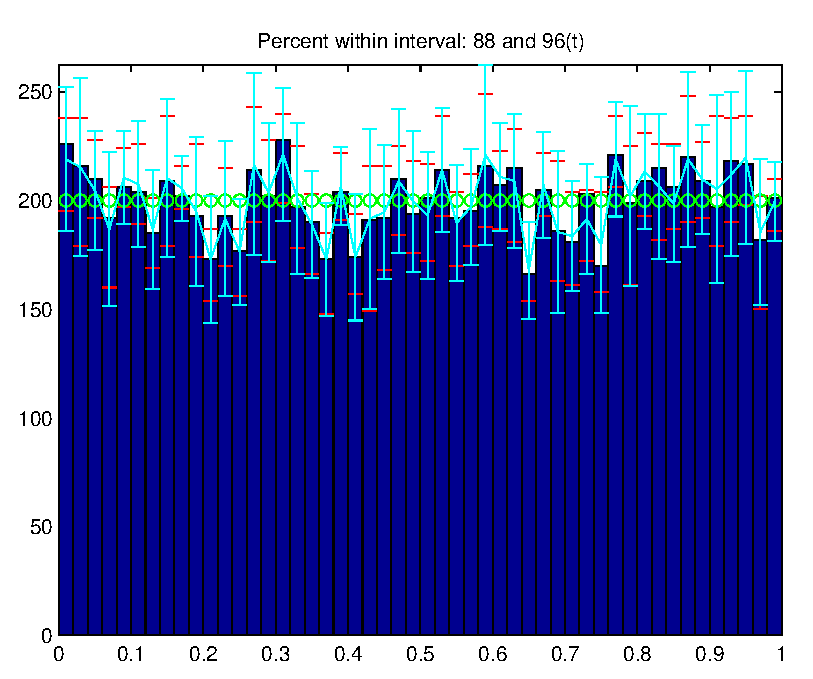
\includegraphics [width=4in]{bootstrapci_01.eps}



\end{document}
    
